\documentclass[twoside]{book}

% Packages required by doxygen
\usepackage{fixltx2e}
\usepackage{calc}
\usepackage{doxygen}
\usepackage[export]{adjustbox} % also loads graphicx
\usepackage{graphicx}
\usepackage[utf8]{inputenc}
\usepackage{makeidx}
\usepackage{multicol}
\usepackage{multirow}
\PassOptionsToPackage{warn}{textcomp}
\usepackage{textcomp}
\usepackage[nointegrals]{wasysym}
\usepackage[table]{xcolor}

% NLS support packages
\usepackage[spanish]{babel}
% Font selection
\usepackage[T1]{fontenc}
\usepackage[scaled=.90]{helvet}
\usepackage{courier}
\usepackage{amssymb}
\usepackage{sectsty}
\renewcommand{\familydefault}{\sfdefault}
\allsectionsfont{%
  \fontseries{bc}\selectfont%
  \color{darkgray}%
}
\renewcommand{\DoxyLabelFont}{%
  \fontseries{bc}\selectfont%
  \color{darkgray}%
}
\newcommand{\+}{\discretionary{\mbox{\scriptsize$\hookleftarrow$}}{}{}}

% Page & text layout
\usepackage{geometry}
\geometry{%
  a4paper,%
  top=2.5cm,%
  bottom=2.5cm,%
  left=2.5cm,%
  right=2.5cm%
}
\tolerance=750
\hfuzz=15pt
\hbadness=750
\setlength{\emergencystretch}{15pt}
\setlength{\parindent}{0cm}
\setlength{\parskip}{3ex plus 2ex minus 2ex}
\makeatletter
\renewcommand{\paragraph}{%
  \@startsection{paragraph}{4}{0ex}{-1.0ex}{1.0ex}{%
    \normalfont\normalsize\bfseries\SS@parafont%
  }%
}
\renewcommand{\subparagraph}{%
  \@startsection{subparagraph}{5}{0ex}{-1.0ex}{1.0ex}{%
    \normalfont\normalsize\bfseries\SS@subparafont%
  }%
}
\makeatother

% Headers & footers
\usepackage{fancyhdr}
\pagestyle{fancyplain}
\fancyhead[LE]{\fancyplain{}{\bfseries\thepage}}
\fancyhead[CE]{\fancyplain{}{}}
\fancyhead[RE]{\fancyplain{}{\bfseries\leftmark}}
\fancyhead[LO]{\fancyplain{}{\bfseries\rightmark}}
\fancyhead[CO]{\fancyplain{}{}}
\fancyhead[RO]{\fancyplain{}{\bfseries\thepage}}
\fancyfoot[LE]{\fancyplain{}{}}
\fancyfoot[CE]{\fancyplain{}{}}
\fancyfoot[RE]{\fancyplain{}{\bfseries\scriptsize Generado por Doxygen }}
\fancyfoot[LO]{\fancyplain{}{\bfseries\scriptsize Generado por Doxygen }}
\fancyfoot[CO]{\fancyplain{}{}}
\fancyfoot[RO]{\fancyplain{}{}}
\renewcommand{\footrulewidth}{0.4pt}
\renewcommand{\chaptermark}[1]{%
  \markboth{#1}{}%
}
\renewcommand{\sectionmark}[1]{%
  \markright{\thesection\ #1}%
}

% Indices & bibliography
\usepackage{natbib}
\usepackage[titles]{tocloft}
\setcounter{tocdepth}{3}
\setcounter{secnumdepth}{5}
\makeindex

% Hyperlinks (required, but should be loaded last)
\usepackage{ifpdf}
\ifpdf
  \usepackage[pdftex,pagebackref=true]{hyperref}
\else
  \usepackage[ps2pdf,pagebackref=true]{hyperref}
\fi
\hypersetup{%
  colorlinks=true,%
  linkcolor=blue,%
  citecolor=blue,%
  unicode%
}

% Custom commands
\newcommand{\clearemptydoublepage}{%
  \newpage{\pagestyle{empty}\cleardoublepage}%
}

\usepackage{caption}
\captionsetup{labelsep=space,justification=centering,font={bf},singlelinecheck=off,skip=4pt,position=top}

%===== C O N T E N T S =====

\begin{document}

% Titlepage & ToC
\hypersetup{pageanchor=false,
             bookmarksnumbered=true,
             pdfencoding=unicode
            }
\pagenumbering{roman}
\begin{titlepage}
\vspace*{7cm}
\begin{center}%
{\Large Práctica 1 -\/ S\+O\+P\+ER }\\
\vspace*{1cm}
{\large Generado por Doxygen 1.8.11}\\
\end{center}
\end{titlepage}
\clearemptydoublepage
\tableofcontents
\clearemptydoublepage
\pagenumbering{arabic}
\hypersetup{pageanchor=true}

%--- Begin generated contents ---
\chapter{Índice de estructura de datos}
\section{Estructura de datos}
Lista de estructuras con una breve descripción\+:\begin{DoxyCompactList}
\item\contentsline{section}{\hyperlink{structmatrix}{matrix} }{\pageref{structmatrix}}{}
\end{DoxyCompactList}

\chapter{Indice de archivos}
\section{Lista de archivos}
Lista de todos los archivos documentados y con descripciones breves\+:\begin{DoxyCompactList}
\item\contentsline{section}{\hyperlink{ejercicio10_8c}{ejercicio10.\+c} \\*Fuente del ejercicio 10 }{\pageref{ejercicio10_8c}}{}
\item\contentsline{section}{\hyperlink{ejercicio10b_8c}{ejercicio10b.\+c} \\*Fuente del ejercicio 10, versión2 }{\pageref{ejercicio10b_8c}}{}
\item\contentsline{section}{\hyperlink{ejercicio3a_8c}{ejercicio3a.\+c} \\*Fuente del ejercicio 3a }{\pageref{ejercicio3a_8c}}{}
\item\contentsline{section}{\hyperlink{ejercicio3b_8c}{ejercicio3b.\+c} \\*Fuente del ejercicio 3b }{\pageref{ejercicio3b_8c}}{}
\item\contentsline{section}{\hyperlink{ejercicio4_8c}{ejercicio4.\+c} \\*Fuente del ejercicio 4 Este programa pide al usuario dos matrices y dos factores para multiplicarlas. Multiplica cada una por un factor en dos hilos distintos que además mantienen una comunicación para saber por donde va el otro }{\pageref{ejercicio4_8c}}{}
\item\contentsline{section}{\hyperlink{ejercicio8_8c}{ejercicio8.\+c} \\*Fuente del ejercicio 8 Este programa pide al usuario un número de procesos y un número de vueltas, estos procesos se pasarán una señal tantas vueltas como pida el usuario. Cada vez que uno la recibe, imprime la hora. Finalmente se acaban uno a uno }{\pageref{ejercicio8_8c}}{}
\end{DoxyCompactList}

\chapter{Documentación de las estructuras de datos}
\hypertarget{structmatrix}{}\section{Referencia de la Estructura matrix}
\label{structmatrix}\index{matrix@{matrix}}
\subsection*{Campos de datos}
\begin{DoxyCompactItemize}
\item 
int {\bfseries dim}\hypertarget{structmatrix_ac555d1f0296d300abae35fd64afe0b87}{}\label{structmatrix_ac555d1f0296d300abae35fd64afe0b87}

\item 
int $\ast$$\ast$ {\bfseries matrix1}\hypertarget{structmatrix_ac24f129df509efe1cd0b54d707fa8071}{}\label{structmatrix_ac24f129df509efe1cd0b54d707fa8071}

\item 
int $\ast$$\ast$ {\bfseries matrix2}\hypertarget{structmatrix_add8a2cdae83ae685f5d120dd52561e6a}{}\label{structmatrix_add8a2cdae83ae685f5d120dd52561e6a}

\item 
int {\bfseries fila1}\hypertarget{structmatrix_a953218c79ce6af792c8f48bda1d490ca}{}\label{structmatrix_a953218c79ce6af792c8f48bda1d490ca}

\item 
int {\bfseries fila2}\hypertarget{structmatrix_abcf3d9279ba1858992b65bcf39f6646a}{}\label{structmatrix_abcf3d9279ba1858992b65bcf39f6646a}

\item 
int {\bfseries mul1}\hypertarget{structmatrix_a650aeaf369809556dcd40e458a02bccd}{}\label{structmatrix_a650aeaf369809556dcd40e458a02bccd}

\item 
int {\bfseries mul2}\hypertarget{structmatrix_a602974f58f94fda7067ada66e2cf56b2}{}\label{structmatrix_a602974f58f94fda7067ada66e2cf56b2}

\end{DoxyCompactItemize}


La documentación para esta estructura fue generada a partir del siguiente fichero\+:\begin{DoxyCompactItemize}
\item 
\hyperlink{ejercicio4_8c}{ejercicio4.\+c}\end{DoxyCompactItemize}

\chapter{Documentación de archivos}
\hypertarget{ejercicio10_8c}{}\section{Referencia del Archivo ejercicio10.\+c}
\label{ejercicio10_8c}\index{ejercicio10.\+c@{ejercicio10.\+c}}


Fuente del ejercicio 10.  


{\ttfamily \#include $<$stdio.\+h$>$}\\*
{\ttfamily \#include $<$stdlib.\+h$>$}\\*
{\ttfamily \#include $<$string.\+h$>$}\\*
{\ttfamily \#include $<$signal.\+h$>$}\\*
{\ttfamily \#include $<$unistd.\+h$>$}\\*
{\ttfamily \#include $<$sys/types.\+h$>$}\\*
{\ttfamily \#include $<$sys/wait.\+h$>$}\\*
{\ttfamily \#include $<$fcntl.\+h$>$}\\*
{\ttfamily \#include $<$time.\+h$>$}\\*
Dependencia gráfica adjunta para ejercicio10.\+c\+:
\nopagebreak
\begin{figure}[H]
\begin{center}
\leavevmode
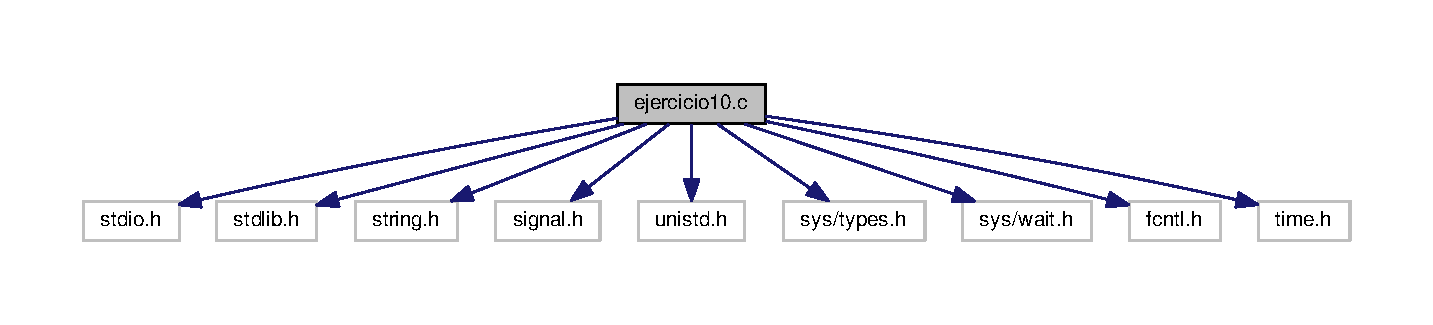
\includegraphics[width=350pt]{ejercicio10_8c__incl}
\end{center}
\end{figure}
\subsection*{\textquotesingle{}defines\textquotesingle{}}
\begin{DoxyCompactItemize}
\item 
\#define {\bfseries M\+A\+X\+B\+UF}~256\hypertarget{ejercicio10_8c_ad7871643c05865c80f5d8050aead2b57}{}\label{ejercicio10_8c_ad7871643c05865c80f5d8050aead2b57}

\end{DoxyCompactItemize}
\subsection*{Funciones}
\begin{DoxyCompactItemize}
\item 
void \hyperlink{ejercicio10_8c_aae89ff4f81b8ee890b1a41ed2a2fab23}{manejador\+\_\+sigalrm} (int sig)
\item 
int {\bfseries main} ()\hypertarget{ejercicio10_8c_ae66f6b31b5ad750f1fe042a706a4e3d4}{}\label{ejercicio10_8c_ae66f6b31b5ad750f1fe042a706a4e3d4}

\end{DoxyCompactItemize}


\subsection{Descripción detallada}
Fuente del ejercicio 10. 

El programa ejercicio10 ejercutará un fork, del resultado del cual el hijo escribirá en un fichero una palabra aleatoria de la frase del enunciado, y si escribe la palabra \char`\"{}\+F\+I\+N\char`\"{} termina su ejecución. El padre esperará 5 segundos y leerá una palabra, si ésta es \char`\"{}\+F\+I\+N\char`\"{}, entenderá que su hijo ha terminado y lo reanimará. Si no, continuará. Este proceso se ejecuta 50 veces.

\begin{DoxyAuthor}{Autor}
Juan Riera Gomez (\href{mailto:juan.riera@estudiante.uam.es}{\tt juan.\+riera@estudiante.\+uam.\+es}) y Carlos Ignacio Isasa Martín (\href{mailto:carlos.isasa@estudiante.uam.es}{\tt carlos.\+isasa@estudiante.\+uam.\+es}) 
\end{DoxyAuthor}
\begin{DoxyVersion}{Versión}
1.\+0 
\end{DoxyVersion}
\begin{DoxyDate}{Fecha}
15-\/03-\/2017 
\end{DoxyDate}


\subsection{Documentación de las funciones}
\index{ejercicio10.\+c@{ejercicio10.\+c}!manejador\+\_\+sigalrm@{manejador\+\_\+sigalrm}}
\index{manejador\+\_\+sigalrm@{manejador\+\_\+sigalrm}!ejercicio10.\+c@{ejercicio10.\+c}}
\subsubsection[{\texorpdfstring{manejador\+\_\+sigalrm(int sig)}{manejador_sigalrm(int sig)}}]{\setlength{\rightskip}{0pt plus 5cm}void manejador\+\_\+sigalrm (
\begin{DoxyParamCaption}
\item[{int}]{sig}
\end{DoxyParamCaption}
)}\hypertarget{ejercicio10_8c_aae89ff4f81b8ee890b1a41ed2a2fab23}{}\label{ejercicio10_8c_aae89ff4f81b8ee890b1a41ed2a2fab23}
Este es el manejador de la señal de alarma de reloj (S\+I\+G\+A\+L\+RM)i que no tiene nada, ya que nos interesa que simplemente espere a la llegada de la señal y continúe su ejecución. 
\hypertarget{ejercicio10b_8c}{}\section{Referencia del Archivo ejercicio10b.\+c}
\label{ejercicio10b_8c}\index{ejercicio10b.\+c@{ejercicio10b.\+c}}


Fuente del ejercicio 10, versión2.  


{\ttfamily \#include $<$stdio.\+h$>$}\\*
{\ttfamily \#include $<$stdlib.\+h$>$}\\*
{\ttfamily \#include $<$string.\+h$>$}\\*
{\ttfamily \#include $<$signal.\+h$>$}\\*
{\ttfamily \#include $<$unistd.\+h$>$}\\*
{\ttfamily \#include $<$sys/types.\+h$>$}\\*
{\ttfamily \#include $<$sys/wait.\+h$>$}\\*
{\ttfamily \#include $<$fcntl.\+h$>$}\\*
{\ttfamily \#include $<$time.\+h$>$}\\*
Dependencia gráfica adjunta para ejercicio10b.\+c\+:
\nopagebreak
\begin{figure}[H]
\begin{center}
\leavevmode
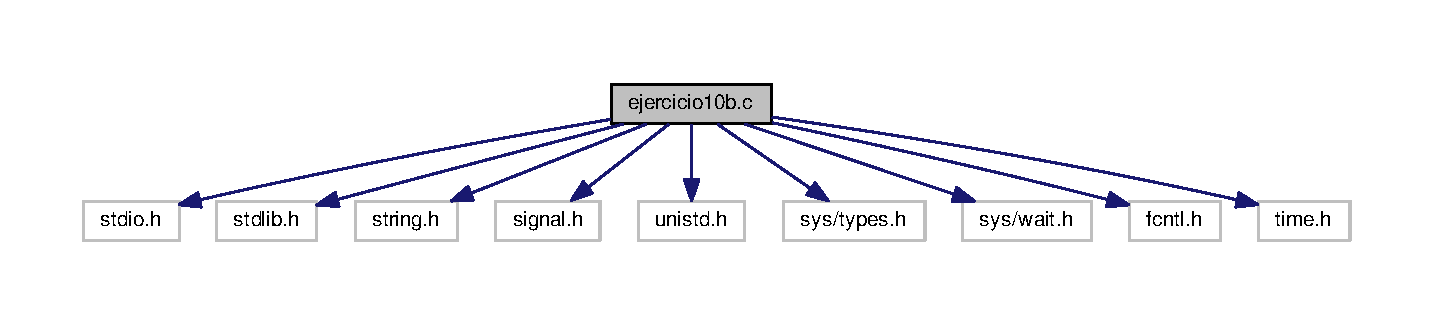
\includegraphics[width=350pt]{ejercicio10b_8c__incl}
\end{center}
\end{figure}
\subsection*{\textquotesingle{}defines\textquotesingle{}}
\begin{DoxyCompactItemize}
\item 
\#define {\bfseries M\+A\+X\+B\+UF}~256\hypertarget{ejercicio10b_8c_ad7871643c05865c80f5d8050aead2b57}{}\label{ejercicio10b_8c_ad7871643c05865c80f5d8050aead2b57}

\end{DoxyCompactItemize}
\subsection*{Funciones}
\begin{DoxyCompactItemize}
\item 
void \hyperlink{ejercicio10b_8c_aae89ff4f81b8ee890b1a41ed2a2fab23}{manejador\+\_\+sigalrm} (int sig)
\item 
int {\bfseries main} ()\hypertarget{ejercicio10b_8c_ae66f6b31b5ad750f1fe042a706a4e3d4}{}\label{ejercicio10b_8c_ae66f6b31b5ad750f1fe042a706a4e3d4}

\end{DoxyCompactItemize}


\subsection{Descripción detallada}
Fuente del ejercicio 10, versión2. 

Este es el ejercicio 10, pero una segunda versión que imprime cada lectura y cada escritura cada vez que se ejecuta, ya que no se especifica ninguna salida por pantalla. Por lo demás no se diferencia en nada del fuente \char`\"{}ejercicio10.\+c\char`\"{}

\begin{DoxyAuthor}{Autor}
Juan Riera Gomez (\href{mailto:juan.riera@estudiante.uam.es}{\tt juan.\+riera@estudiante.\+uam.\+es}) y Carlos Ignacio Isasa Martín (\href{mailto:carlos.isasa@estudiante.uam.es}{\tt carlos.\+isasa@estudiante.\+uam.\+es}) 
\end{DoxyAuthor}
\begin{DoxyVersion}{Versión}
2.\+0 
\end{DoxyVersion}
\begin{DoxyDate}{Fecha}
15-\/03-\/2017 
\end{DoxyDate}


\subsection{Documentación de las funciones}
\index{ejercicio10b.\+c@{ejercicio10b.\+c}!manejador\+\_\+sigalrm@{manejador\+\_\+sigalrm}}
\index{manejador\+\_\+sigalrm@{manejador\+\_\+sigalrm}!ejercicio10b.\+c@{ejercicio10b.\+c}}
\subsubsection[{\texorpdfstring{manejador\+\_\+sigalrm(int sig)}{manejador_sigalrm(int sig)}}]{\setlength{\rightskip}{0pt plus 5cm}void manejador\+\_\+sigalrm (
\begin{DoxyParamCaption}
\item[{int}]{sig}
\end{DoxyParamCaption}
)}\hypertarget{ejercicio10b_8c_aae89ff4f81b8ee890b1a41ed2a2fab23}{}\label{ejercicio10b_8c_aae89ff4f81b8ee890b1a41ed2a2fab23}
Este es el manejador de la señal de alarma de reloj (S\+I\+G\+A\+L\+RM)i que no tiene nada, ya que nos interesa que simplemente espere a la llegada de la señal y continúe su ejecución. 
\hypertarget{ejercicio3a_8c}{}\section{Referencia del Archivo ejercicio3a.\+c}
\label{ejercicio3a_8c}\index{ejercicio3a.\+c@{ejercicio3a.\+c}}


Fuente del ejercicio 3a.  


{\ttfamily \#include $<$stdio.\+h$>$}\\*
{\ttfamily \#include $<$stdlib.\+h$>$}\\*
{\ttfamily \#include $<$unistd.\+h$>$}\\*
{\ttfamily \#include $<$string.\+h$>$}\\*
{\ttfamily \#include $<$sys/time.\+h$>$}\\*
{\ttfamily \#include $<$sys/types.\+h$>$}\\*
{\ttfamily \#include $<$sys/wait.\+h$>$}\\*
{\ttfamily \#include $<$limits.\+h$>$}\\*
Dependencia gráfica adjunta para ejercicio3a.\+c\+:
\nopagebreak
\begin{figure}[H]
\begin{center}
\leavevmode
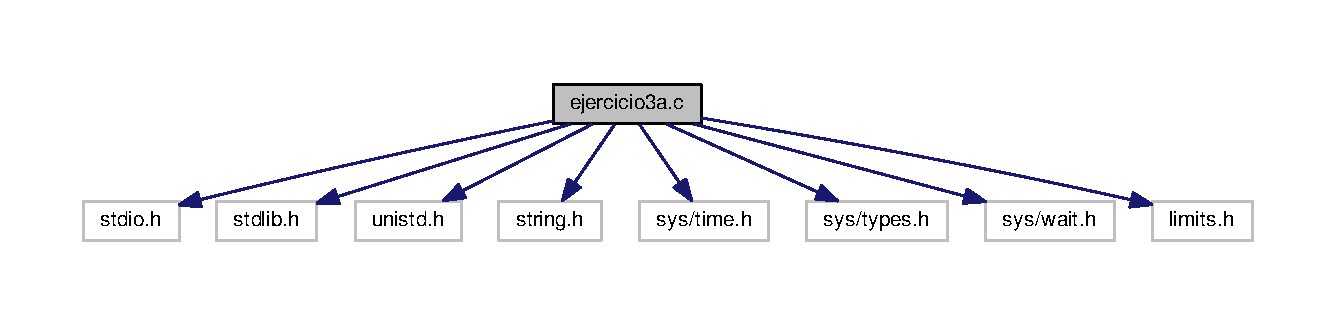
\includegraphics[width=350pt]{ejercicio3a_8c__incl}
\end{center}
\end{figure}
\subsection*{\textquotesingle{}defines\textquotesingle{}}
\begin{DoxyCompactItemize}
\item 
\#define {\bfseries N\+U\+M\+P\+R\+OC}~100\hypertarget{ejercicio3a_8c_a6918fedc593652387b93ea5832745bbb}{}\label{ejercicio3a_8c_a6918fedc593652387b93ea5832745bbb}

\end{DoxyCompactItemize}
\subsection*{Funciones}
\begin{DoxyCompactItemize}
\item 
void $\ast$ \hyperlink{ejercicio3a_8c_a6be374870e70ff630544dfbbca42cf85}{calcula\+Primos} (void $\ast$arg)
\item 
int {\bfseries main} (int argc, char $\ast$$\ast$argv)\hypertarget{ejercicio3a_8c_a3c04138a5bfe5d72780bb7e82a18e627}{}\label{ejercicio3a_8c_a3c04138a5bfe5d72780bb7e82a18e627}

\end{DoxyCompactItemize}


\subsection{Descripción detallada}
Fuente del ejercicio 3a. 

Fuente del ejercicio 6.

Este programa crea un numero de procesos hijo (definido por N\+U\+M\+P\+R\+OC) y cada uno de éstos llama a la funcion calcula\+Primos, que recibe como argumento el número de primos a calcular, y calcula ese número de primos.

\begin{DoxyAuthor}{Autor}
Juan Riera Gomez (\href{mailto:juan.riera@estudiante.uam.es}{\tt juan.\+riera@estudiante.\+uam.\+es}) y Carlos Ignacio Isasa Martín (\href{mailto:carlos.isasa@estudiante.uam.es}{\tt carlos.\+isasa@estudiante.\+uam.\+es}) 
\end{DoxyAuthor}
\begin{DoxyVersion}{Versión}
1.\+0 
\end{DoxyVersion}
\begin{DoxyDate}{Fecha}
15-\/03-\/2017
\end{DoxyDate}
Este programa crea un proceso hijo que escribe por pantalla y espera 5 segundos. El proceso padre espera 30 y mata al proceso hijo.

\begin{DoxyAuthor}{Autor}
Juan Riera Gomez (\href{mailto:juan.riera@estudiante.uam.es}{\tt juan.\+riera@estudiante.\+uam.\+es}) y Carlos Ignacio Isasa Martín (\href{mailto:carlos.isasa@estudiante.uam.es}{\tt carlos.\+isasa@estudiante.\+uam.\+es}) 
\end{DoxyAuthor}
\begin{DoxyVersion}{Versión}
1.\+0 
\end{DoxyVersion}
\begin{DoxyDate}{Fecha}
15-\/03-\/2017 
\end{DoxyDate}


\subsection{Documentación de las funciones}
\index{ejercicio3a.\+c@{ejercicio3a.\+c}!calcula\+Primos@{calcula\+Primos}}
\index{calcula\+Primos@{calcula\+Primos}!ejercicio3a.\+c@{ejercicio3a.\+c}}
\subsubsection[{\texorpdfstring{calcula\+Primos(void $\ast$arg)}{calculaPrimos(void *arg)}}]{\setlength{\rightskip}{0pt plus 5cm}void$\ast$ calcula\+Primos (
\begin{DoxyParamCaption}
\item[{void $\ast$}]{arg}
\end{DoxyParamCaption}
)}\hypertarget{ejercicio3a_8c_a6be374870e70ff630544dfbbca42cf85}{}\label{ejercicio3a_8c_a6be374870e70ff630544dfbbca42cf85}
Función calcula primos\+: Calcula un número entero de números primos que recibe por parámetros. 
\begin{DoxyParams}{Parámetros}
{\em (void$\ast$)(int} & arg)\+: número de primos a calular \\
\hline
\end{DoxyParams}

\hypertarget{ejercicio3b_8c}{}\section{Referencia del Archivo ejercicio3b.\+c}
\label{ejercicio3b_8c}\index{ejercicio3b.\+c@{ejercicio3b.\+c}}


Fuente del ejercicio 3b.  


{\ttfamily \#include $<$stdio.\+h$>$}\\*
{\ttfamily \#include $<$stdlib.\+h$>$}\\*
{\ttfamily \#include $<$unistd.\+h$>$}\\*
{\ttfamily \#include $<$string.\+h$>$}\\*
{\ttfamily \#include $<$sys/time.\+h$>$}\\*
{\ttfamily \#include $<$sys/types.\+h$>$}\\*
{\ttfamily \#include $<$sys/wait.\+h$>$}\\*
{\ttfamily \#include $<$limits.\+h$>$}\\*
{\ttfamily \#include $<$pthread.\+h$>$}\\*
Dependencia gráfica adjunta para ejercicio3b.\+c\+:
\nopagebreak
\begin{figure}[H]
\begin{center}
\leavevmode
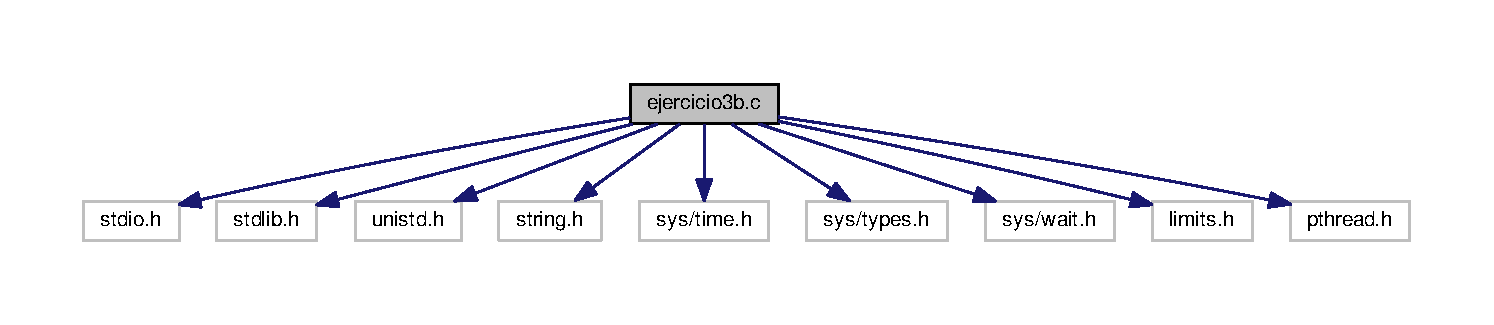
\includegraphics[width=350pt]{ejercicio3b_8c__incl}
\end{center}
\end{figure}
\subsection*{\textquotesingle{}defines\textquotesingle{}}
\begin{DoxyCompactItemize}
\item 
\#define {\bfseries N\+U\+M\+T\+H\+R\+E\+AD}~100\hypertarget{ejercicio3b_8c_a25077975290fe3ab631d565e49cb73ba}{}\label{ejercicio3b_8c_a25077975290fe3ab631d565e49cb73ba}

\end{DoxyCompactItemize}
\subsection*{Funciones}
\begin{DoxyCompactItemize}
\item 
void $\ast$ \hyperlink{ejercicio3b_8c_a6be374870e70ff630544dfbbca42cf85}{calcula\+Primos} (void $\ast$arg)
\item 
int {\bfseries main} (int argc, char $\ast$$\ast$argv)\hypertarget{ejercicio3b_8c_a3c04138a5bfe5d72780bb7e82a18e627}{}\label{ejercicio3b_8c_a3c04138a5bfe5d72780bb7e82a18e627}

\end{DoxyCompactItemize}


\subsection{Descripción detallada}
Fuente del ejercicio 3b. 

Este programa crea un numero de hilos hijo (definido por N\+U\+M\+T\+H\+R\+E\+AD) y cada uno de éstos llama a la funcion calcula\+Primos, que recibe como argumento el número de primos a calcular, y calcula ese número de primos.

\begin{DoxyAuthor}{Autor}
Juan Riera Gomez (\href{mailto:juan.riera@estudiante.uam.es}{\tt juan.\+riera@estudiante.\+uam.\+es}) y Carlos Ignacio Isasa Martín (\href{mailto:carlos.isasa@estudiante.uam.es}{\tt carlos.\+isasa@estudiante.\+uam.\+es}) 
\end{DoxyAuthor}
\begin{DoxyVersion}{Versión}
1.\+0 
\end{DoxyVersion}
\begin{DoxyDate}{Fecha}
15-\/03-\/2017 
\end{DoxyDate}


\subsection{Documentación de las funciones}
\index{ejercicio3b.\+c@{ejercicio3b.\+c}!calcula\+Primos@{calcula\+Primos}}
\index{calcula\+Primos@{calcula\+Primos}!ejercicio3b.\+c@{ejercicio3b.\+c}}
\subsubsection[{\texorpdfstring{calcula\+Primos(void $\ast$arg)}{calculaPrimos(void *arg)}}]{\setlength{\rightskip}{0pt plus 5cm}void$\ast$ calcula\+Primos (
\begin{DoxyParamCaption}
\item[{void $\ast$}]{arg}
\end{DoxyParamCaption}
)}\hypertarget{ejercicio3b_8c_a6be374870e70ff630544dfbbca42cf85}{}\label{ejercicio3b_8c_a6be374870e70ff630544dfbbca42cf85}
Función calcula primos\+: Calcula un número entero de números primos que recibe por parámetros. 
\begin{DoxyParams}{Parámetros}
{\em (void$\ast$)(int} & arg)\+: número de primos a calular \\
\hline
\end{DoxyParams}

\hypertarget{ejercicio4_8c}{}\section{Referencia del Archivo ejercicio4.\+c}
\label{ejercicio4_8c}\index{ejercicio4.\+c@{ejercicio4.\+c}}


Fuente del ejercicio 4 Este programa pide al usuario dos matrices y dos factores para multiplicarlas. Multiplica cada una por un factor en dos hilos distintos que además mantienen una comunicación para saber por donde va el otro.  


{\ttfamily \#include $<$stdio.\+h$>$}\\*
{\ttfamily \#include $<$stdlib.\+h$>$}\\*
{\ttfamily \#include $<$unistd.\+h$>$}\\*
{\ttfamily \#include $<$string.\+h$>$}\\*
{\ttfamily \#include $<$pthread.\+h$>$}\\*
Dependencia gráfica adjunta para ejercicio4.\+c\+:
\nopagebreak
\begin{figure}[H]
\begin{center}
\leavevmode
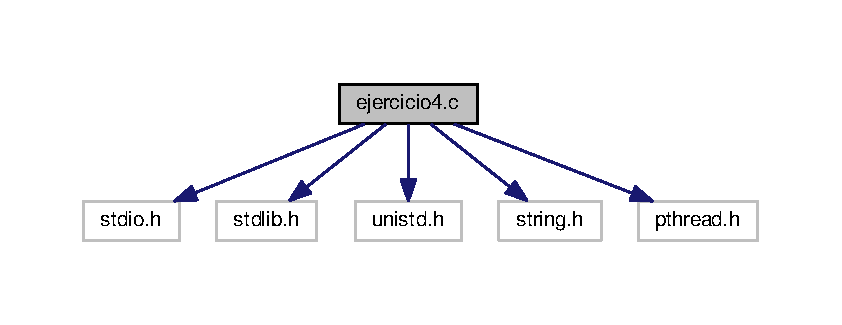
\includegraphics[width=350pt]{ejercicio4_8c__incl}
\end{center}
\end{figure}
\subsection*{Estructuras de datos}
\begin{DoxyCompactItemize}
\item 
struct \hyperlink{structmatrix}{matrix}
\end{DoxyCompactItemize}
\subsection*{\textquotesingle{}typedefs\textquotesingle{}}
\begin{DoxyCompactItemize}
\item 
typedef struct \hyperlink{structmatrix}{matrix} {\bfseries Matrix}\hypertarget{ejercicio4_8c_a9a1246023f40a820ce7ac97a61b8d4e0}{}\label{ejercicio4_8c_a9a1246023f40a820ce7ac97a61b8d4e0}

\end{DoxyCompactItemize}
\subsection*{Funciones}
\begin{DoxyCompactItemize}
\item 
\hyperlink{structmatrix}{Matrix} $\ast$ {\bfseries matrix\+\_\+create} (int dim, int mul1, int mul2, char $\ast$matrix1, char $\ast$matrix2)\hypertarget{ejercicio4_8c_aff8a75e7d6bcd60ae075774d9f6094d0}{}\label{ejercicio4_8c_aff8a75e7d6bcd60ae075774d9f6094d0}

\item 
void {\bfseries matrix\+\_\+print} (\hyperlink{structmatrix}{Matrix} $\ast$m)\hypertarget{ejercicio4_8c_a61925e6538cbcdb2d1be0455df31078d}{}\label{ejercicio4_8c_a61925e6538cbcdb2d1be0455df31078d}

\item 
void {\bfseries matrix\+\_\+free} (\hyperlink{structmatrix}{Matrix} $\ast$m)\hypertarget{ejercicio4_8c_a8e7cf1507ce317450f07737f4c5c6638}{}\label{ejercicio4_8c_a8e7cf1507ce317450f07737f4c5c6638}

\item 
void $\ast$ {\bfseries first\+\_\+matrix} (void $\ast$\hyperlink{structmatrix}{matrix})\hypertarget{ejercicio4_8c_a2447e77b228ae6cce3c32c6769557fc4}{}\label{ejercicio4_8c_a2447e77b228ae6cce3c32c6769557fc4}

\item 
void $\ast$ {\bfseries second\+\_\+matrix} (void $\ast$\hyperlink{structmatrix}{matrix})\hypertarget{ejercicio4_8c_a447c6f40c750f2662ca19c510951ac6c}{}\label{ejercicio4_8c_a447c6f40c750f2662ca19c510951ac6c}

\item 
int {\bfseries main} ()\hypertarget{ejercicio4_8c_ae66f6b31b5ad750f1fe042a706a4e3d4}{}\label{ejercicio4_8c_ae66f6b31b5ad750f1fe042a706a4e3d4}

\end{DoxyCompactItemize}


\subsection{Descripción detallada}
Fuente del ejercicio 4 Este programa pide al usuario dos matrices y dos factores para multiplicarlas. Multiplica cada una por un factor en dos hilos distintos que además mantienen una comunicación para saber por donde va el otro. 

\begin{DoxyAuthor}{Autor}
Juan Riera Gomez (\href{mailto:juan.riera@estudiante.uam.es}{\tt juan.\+riera@estudiante.\+uam.\+es}) y Carlos Ignacio Isasa Martín (\href{mailto:carlos.isasa@estudiante.uam.es}{\tt carlos.\+isasa@estudiante.\+uam.\+es}) 
\end{DoxyAuthor}
\begin{DoxyVersion}{Versión}
1.\+0 
\end{DoxyVersion}
\begin{DoxyDate}{Fecha}
14-\/03-\/2017 
\end{DoxyDate}

\hypertarget{ejercicio8_8c}{}\section{Referencia del Archivo ejercicio8.\+c}
\label{ejercicio8_8c}\index{ejercicio8.\+c@{ejercicio8.\+c}}


Fuente del ejercicio 8 Este programa pide al usuario un número de procesos y un número de vueltas, estos procesos se pasarán una señal tantas vueltas como pida el usuario. Cada vez que uno la recibe, imprime la hora. Finalmente se acaban uno a uno.  


{\ttfamily \#include $<$stdio.\+h$>$}\\*
{\ttfamily \#include $<$stdlib.\+h$>$}\\*
{\ttfamily \#include $<$string.\+h$>$}\\*
{\ttfamily \#include $<$signal.\+h$>$}\\*
{\ttfamily \#include $<$unistd.\+h$>$}\\*
{\ttfamily \#include $<$sys/types.\+h$>$}\\*
{\ttfamily \#include $<$sys/wait.\+h$>$}\\*
{\ttfamily \#include $<$fcntl.\+h$>$}\\*
{\ttfamily \#include $<$time.\+h$>$}\\*
Dependencia gráfica adjunta para ejercicio8.\+c\+:
\nopagebreak
\begin{figure}[H]
\begin{center}
\leavevmode
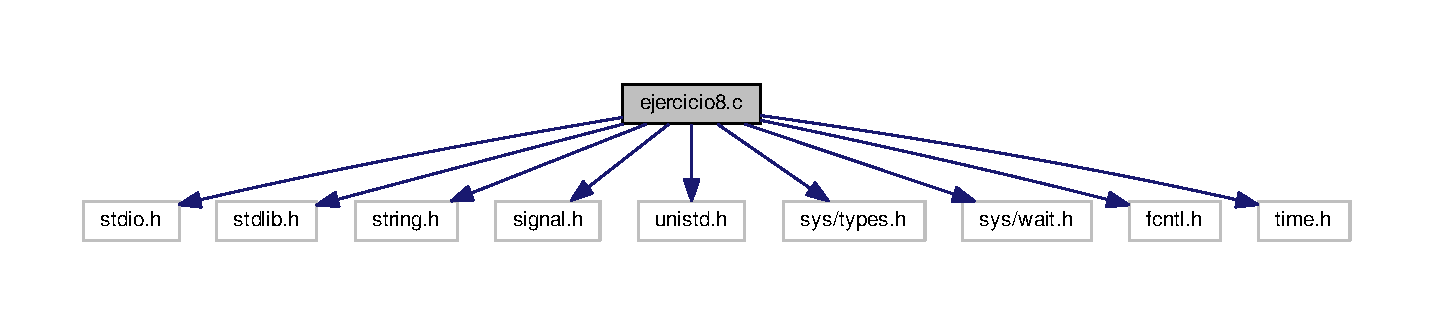
\includegraphics[width=350pt]{ejercicio8_8c__incl}
\end{center}
\end{figure}
\subsection*{Funciones}
\begin{DoxyCompactItemize}
\item 
char $\ast$ {\bfseries tiempo} ()\hypertarget{ejercicio8_8c_a445d4e4144b10aa987da413343200688}{}\label{ejercicio8_8c_a445d4e4144b10aa987da413343200688}

\item 
void {\bfseries manejador\+\_\+sigusr1} (int sig)\hypertarget{ejercicio8_8c_a54e0d453acd2cb0d8adfd611e4158462}{}\label{ejercicio8_8c_a54e0d453acd2cb0d8adfd611e4158462}

\item 
void {\bfseries manejador\+\_\+sigterm} (int sig)\hypertarget{ejercicio8_8c_a7e0d11f7ea2fd257c747e1cea963f357}{}\label{ejercicio8_8c_a7e0d11f7ea2fd257c747e1cea963f357}

\item 
int {\bfseries main} (int argc, char $\ast$argv\mbox{[}$\,$\mbox{]})\hypertarget{ejercicio8_8c_a0ddf1224851353fc92bfbff6f499fa97}{}\label{ejercicio8_8c_a0ddf1224851353fc92bfbff6f499fa97}

\end{DoxyCompactItemize}


\subsection{Descripción detallada}
Fuente del ejercicio 8 Este programa pide al usuario un número de procesos y un número de vueltas, estos procesos se pasarán una señal tantas vueltas como pida el usuario. Cada vez que uno la recibe, imprime la hora. Finalmente se acaban uno a uno. 

\begin{DoxyAuthor}{Autor}
Juan Riera Gomez (\href{mailto:juan.riera@estudiante.uam.es}{\tt juan.\+riera@estudiante.\+uam.\+es}) y Carlos Ignacio Isasa Martín (\href{mailto:carlos.isasa@estudiante.uam.es}{\tt carlos.\+isasa@estudiante.\+uam.\+es}) 
\end{DoxyAuthor}
\begin{DoxyVersion}{Versión}
1.\+0 
\end{DoxyVersion}
\begin{DoxyDate}{Fecha}
15-\/03-\/2017 
\end{DoxyDate}

%--- End generated contents ---

% Index
\backmatter
\newpage
\phantomsection
\clearemptydoublepage
\addcontentsline{toc}{chapter}{Índice}
\printindex

\end{document}
